% Options for packages loaded elsewhere
% Options for packages loaded elsewhere
\PassOptionsToPackage{unicode}{hyperref}
\PassOptionsToPackage{hyphens}{url}
%
\documentclass[
  ignorenonframetext,
  aspectratio=169,
  russian,
]{beamer}
\newif\ifbibliography
\usepackage{pgfpages}
\setbeamertemplate{caption}[numbered]
\setbeamertemplate{caption label separator}{: }
\setbeamercolor{caption name}{fg=normal text.fg}
\beamertemplatenavigationsymbolshorizontal
% Prevent slide breaks in the middle of a paragraph
\widowpenalties 1 10000
\raggedbottom
\AtBeginPart{
  \frame{\partpage}
}
\AtBeginSection{
  \ifbibliography
  \else
    \frame{\sectionpage}
  \fi
}
\AtBeginSubsection{
  \frame{\subsectionpage}
}
\usepackage{iftex}
\ifPDFTeX
  \usepackage[T1]{fontenc}
  \usepackage[utf8]{inputenc}
  \usepackage{textcomp} % provide euro and other symbols
\else % if luatex or xetex
  \usepackage{unicode-math} % this also loads fontspec
  \defaultfontfeatures{Scale=MatchLowercase}
  \defaultfontfeatures[\rmfamily]{Ligatures=TeX,Scale=1}
\fi
\usepackage{lmodern}

\usetheme[]{Montpellier}
\usecolortheme[]{seagull}
\ifPDFTeX\else
  % xetex/luatex font selection
\fi
% Use upquote if available, for straight quotes in verbatim environments
\IfFileExists{upquote.sty}{\usepackage{upquote}}{}
\IfFileExists{microtype.sty}{% use microtype if available
  \usepackage[]{microtype}
  \UseMicrotypeSet[protrusion]{basicmath} % disable protrusion for tt fonts
}{}

\usepackage{color}
\usepackage{fancyvrb}
\newcommand{\VerbBar}{|}
\newcommand{\VERB}{\Verb[commandchars=\\\{\}]}
\DefineVerbatimEnvironment{Highlighting}{Verbatim}{commandchars=\\\{\}}
% Add ',fontsize=\small' for more characters per line
\usepackage{framed}
\definecolor{shadecolor}{RGB}{241,243,245}
\newenvironment{Shaded}{\begin{snugshade}}{\end{snugshade}}
\newcommand{\AlertTok}[1]{\textcolor[rgb]{0.68,0.00,0.00}{#1}}
\newcommand{\AnnotationTok}[1]{\textcolor[rgb]{0.37,0.37,0.37}{#1}}
\newcommand{\AttributeTok}[1]{\textcolor[rgb]{0.40,0.45,0.13}{#1}}
\newcommand{\BaseNTok}[1]{\textcolor[rgb]{0.68,0.00,0.00}{#1}}
\newcommand{\BuiltInTok}[1]{\textcolor[rgb]{0.00,0.23,0.31}{#1}}
\newcommand{\CharTok}[1]{\textcolor[rgb]{0.13,0.47,0.30}{#1}}
\newcommand{\CommentTok}[1]{\textcolor[rgb]{0.37,0.37,0.37}{#1}}
\newcommand{\CommentVarTok}[1]{\textcolor[rgb]{0.37,0.37,0.37}{\textit{#1}}}
\newcommand{\ConstantTok}[1]{\textcolor[rgb]{0.56,0.35,0.01}{#1}}
\newcommand{\ControlFlowTok}[1]{\textcolor[rgb]{0.00,0.23,0.31}{\textbf{#1}}}
\newcommand{\DataTypeTok}[1]{\textcolor[rgb]{0.68,0.00,0.00}{#1}}
\newcommand{\DecValTok}[1]{\textcolor[rgb]{0.68,0.00,0.00}{#1}}
\newcommand{\DocumentationTok}[1]{\textcolor[rgb]{0.37,0.37,0.37}{\textit{#1}}}
\newcommand{\ErrorTok}[1]{\textcolor[rgb]{0.68,0.00,0.00}{#1}}
\newcommand{\ExtensionTok}[1]{\textcolor[rgb]{0.00,0.23,0.31}{#1}}
\newcommand{\FloatTok}[1]{\textcolor[rgb]{0.68,0.00,0.00}{#1}}
\newcommand{\FunctionTok}[1]{\textcolor[rgb]{0.28,0.35,0.67}{#1}}
\newcommand{\ImportTok}[1]{\textcolor[rgb]{0.00,0.46,0.62}{#1}}
\newcommand{\InformationTok}[1]{\textcolor[rgb]{0.37,0.37,0.37}{#1}}
\newcommand{\KeywordTok}[1]{\textcolor[rgb]{0.00,0.23,0.31}{\textbf{#1}}}
\newcommand{\NormalTok}[1]{\textcolor[rgb]{0.00,0.23,0.31}{#1}}
\newcommand{\OperatorTok}[1]{\textcolor[rgb]{0.37,0.37,0.37}{#1}}
\newcommand{\OtherTok}[1]{\textcolor[rgb]{0.00,0.23,0.31}{#1}}
\newcommand{\PreprocessorTok}[1]{\textcolor[rgb]{0.68,0.00,0.00}{#1}}
\newcommand{\RegionMarkerTok}[1]{\textcolor[rgb]{0.00,0.23,0.31}{#1}}
\newcommand{\SpecialCharTok}[1]{\textcolor[rgb]{0.37,0.37,0.37}{#1}}
\newcommand{\SpecialStringTok}[1]{\textcolor[rgb]{0.13,0.47,0.30}{#1}}
\newcommand{\StringTok}[1]{\textcolor[rgb]{0.13,0.47,0.30}{#1}}
\newcommand{\VariableTok}[1]{\textcolor[rgb]{0.07,0.07,0.07}{#1}}
\newcommand{\VerbatimStringTok}[1]{\textcolor[rgb]{0.13,0.47,0.30}{#1}}
\newcommand{\WarningTok}[1]{\textcolor[rgb]{0.37,0.37,0.37}{\textit{#1}}}

\usepackage{longtable,booktabs,array}
\usepackage{calc} % for calculating minipage widths
\usepackage{caption}
% Make caption package work with longtable
\makeatletter
\def\fnum@table{\tablename~\thetable}
\makeatother
\usepackage{graphicx}
\makeatletter
\newsavebox\pandoc@box
\newcommand*\pandocbounded[1]{% scales image to fit in text height/width
  \sbox\pandoc@box{#1}%
  \Gscale@div\@tempa{\textheight}{\dimexpr\ht\pandoc@box+\dp\pandoc@box\relax}%
  \Gscale@div\@tempb{\linewidth}{\wd\pandoc@box}%
  \ifdim\@tempb\p@<\@tempa\p@\let\@tempa\@tempb\fi% select the smaller of both
  \ifdim\@tempa\p@<\p@\scalebox{\@tempa}{\usebox\pandoc@box}%
  \else\usebox{\pandoc@box}%
  \fi%
}
% Set default figure placement to htbp
\def\fps@figure{htbp}
\makeatother



\ifLuaTeX
\usepackage[bidi=basic,provide=*]{babel}
\else
\usepackage[bidi=default,provide=*]{babel}
\fi
% get rid of language-specific shorthands (see #6817):
\let\LanguageShortHands\languageshorthands
\def\languageshorthands#1{}


\setlength{\emergencystretch}{3em} % prevent overfull lines

\providecommand{\tightlist}{%
  \setlength{\itemsep}{0pt}\setlength{\parskip}{0pt}}



 

\usepackage[]{csquotes}

\usepackage{libertine}
\makeatletter
\@ifpackageloaded{caption}{}{\usepackage{caption}}
\AtBeginDocument{%
\ifdefined\contentsname
  \renewcommand*\contentsname{Содержание}
\else
  \newcommand\contentsname{Содержание}
\fi
\ifdefined\listfigurename
  \renewcommand*\listfigurename{Список иллюстраций}
\else
  \newcommand\listfigurename{Список иллюстраций}
\fi
\ifdefined\listtablename
  \renewcommand*\listtablename{Список таблиц}
\else
  \newcommand\listtablename{Список таблиц}
\fi
\ifdefined\figurename
  \renewcommand*\figurename{Рисунок}
\else
  \newcommand\figurename{Рисунок}
\fi
\ifdefined\tablename
  \renewcommand*\tablename{Таблица}
\else
  \newcommand\tablename{Таблица}
\fi
}
\@ifpackageloaded{float}{}{\usepackage{float}}
\floatstyle{ruled}
\@ifundefined{c@chapter}{\newfloat{codelisting}{h}{lop}}{\newfloat{codelisting}{h}{lop}[chapter]}
\floatname{codelisting}{Список}
\newcommand*\listoflistings{\listof{codelisting}{Листинги}}
\makeatother
\makeatletter
\makeatother
\makeatletter
\@ifpackageloaded{caption}{}{\usepackage{caption}}
\@ifpackageloaded{subcaption}{}{\usepackage{subcaption}}
\makeatother

\usepackage{bookmark}
\IfFileExists{xurl.sty}{\usepackage{xurl}}{} % add URL line breaks if available
\urlstyle{same}
\hypersetup{
  pdftitle={Лабораторная работа №1},
  pdfauthor={Мохамед Муса},
  pdflang={ru-RU},
  hidelinks,
  pdfcreator={LaTeX via pandoc}}


\title{Лабораторная работа №1}
\subtitle{Настройка современного окружения разработки}
\author{Мохамед Муса}
\date{2025-10-13}

\begin{document}
\frame{\titlepage}

\renewcommand*\contentsname{Содержание}
\begin{frame}[allowframebreaks]
  \frametitle{Содержание}
  \setcounter{tocdepth}{2}
  \tableofcontents
\end{frame}
\setcounter{tocdepth}{2}
\tableofcontents
}

\begin{frame}{1. Цель и задачи}
\phantomsection\label{ux446ux435ux43bux44c-ux438-ux437ux430ux434ux430ux447ux438}
\begin{block}{1.1 Цель работы}
\phantomsection\label{ux446ux435ux43bux44c-ux440ux430ux431ux43eux442ux44b}
Изучить процесс установки операционной системы Linux (Fedora) в
виртуальной машине, получить практические навыки работы с системой,
освоить базовые команды и принципы администрирования пользователей.
\end{block}
\end{frame}

\begin{columns}[c]
\begin{column}{0.7\linewidth}
\begin{frame}{2. Создание виртуальной машины}
\phantomsection\label{ux441ux43eux437ux434ux430ux43dux438ux435-ux432ux438ux440ux442ux443ux430ux43bux44cux43dux43eux439-ux43cux430ux448ux438ux43dux44b}
\begin{block}{2.1 Настройка виртуальной машины}
\phantomsection\label{ux43dux430ux441ux442ux440ux43eux439ux43aux430-ux432ux438ux440ux442ux443ux430ux43bux44cux43dux43eux439-ux43cux430ux448ux438ux43dux44b}
\begin{itemize}[<+->]
\tightlist
\item
  Создана виртуальная машина в Hyper-V
\item
  Название: \enquote{Fedora}
\item
  Настроены параметры оборудования:

  \begin{itemize}[<+->]
  \tightlist
  \item
    Процессор
  \item
    Оперативная память
  \item
    Жесткий диск
  \item
    Сетевой адаптер`
  \end{itemize}
\end{itemize}
\end{block}
\end{frame}
\end{column}

\begin{column}{0.3\linewidth}
\begin{figure}

\centering{

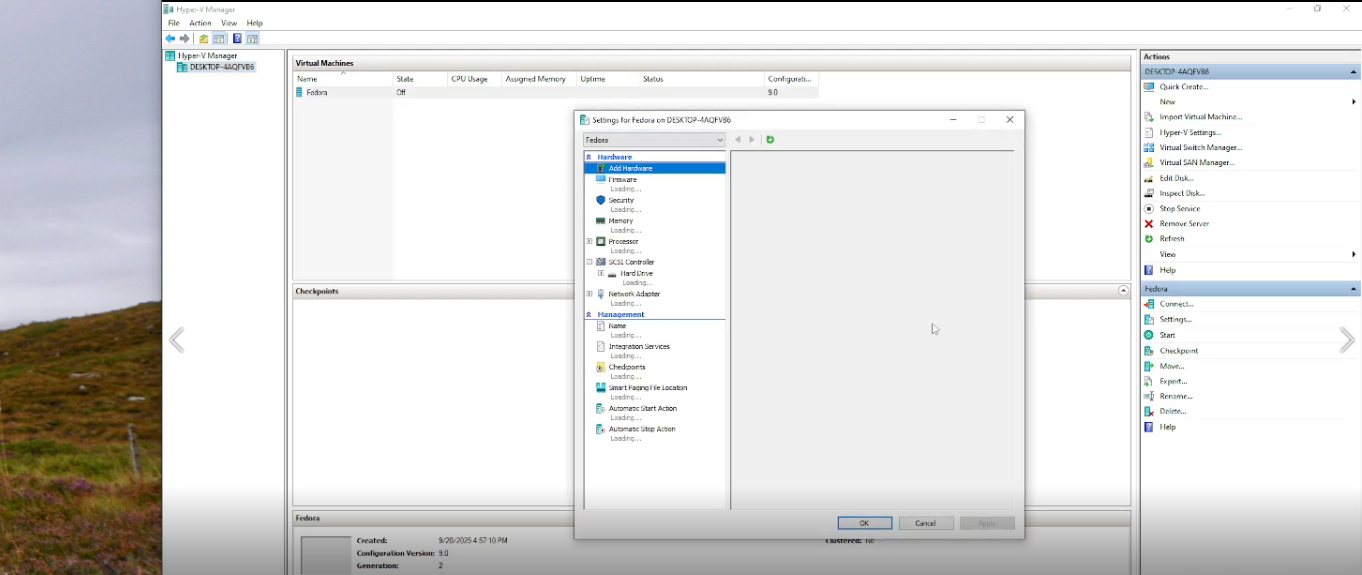
\includegraphics[width=0.9\linewidth,height=\textheight,keepaspectratio]{image/making_vm.PNG}

}

\caption{\label{fig-vm}Создание виртуальной машины}

\end{figure}%
\end{column}
\end{columns}

\begin{block}{2.2 Установка Fedora Linux}
\phantomsection\label{ux443ux441ux442ux430ux43dux43eux432ux43aux430-fedora-linux}
\begin{columns}[c]
\begin{column}{0.7\linewidth}
\begin{itemize}[<+->]
\tightlist
\item
  Загружена live-система Fedora
\item
  Произведена установка ОС
\item
  Настроен язык системы
\item
  Создан пользователь при установке
\end{itemize}
\end{column}

\begin{column}{0.3\linewidth}
\begin{figure}

\centering{

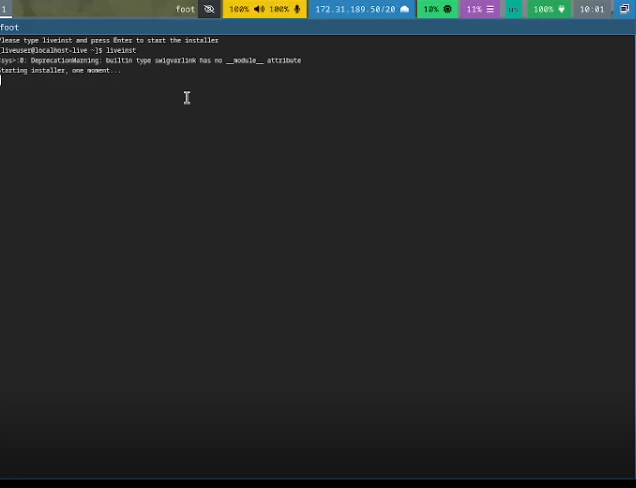
\includegraphics[width=0.9\linewidth,height=\textheight,keepaspectratio]{image/liveinst.PNG}

}

\caption{\label{fig-install}Процесс установки}

\end{figure}%
\end{column}
\end{columns}
\end{block}

\begin{frame}[fragile]{3. Настройка системы}
\phantomsection\label{ux43dux430ux441ux442ux440ux43eux439ux43aux430-ux441ux438ux441ux442ux435ux43cux44b}
\begin{block}{3.1 Создание учетной записи}
\phantomsection\label{ux441ux43eux437ux434ux430ux43dux438ux435-ux443ux447ux435ux442ux43dux43eux439-ux437ux430ux43fux438ux441ux438}
\begin{columns}[c]
\begin{column}{0.7\linewidth}
\textbf{Команды настройки пользователя:} - Создание пользователя и
добавление в группу wheel - Установка полного имени пользователя -
Настройка прав доступа
\end{column}

\begin{column}{0.3\linewidth}
\begin{figure}

\centering{

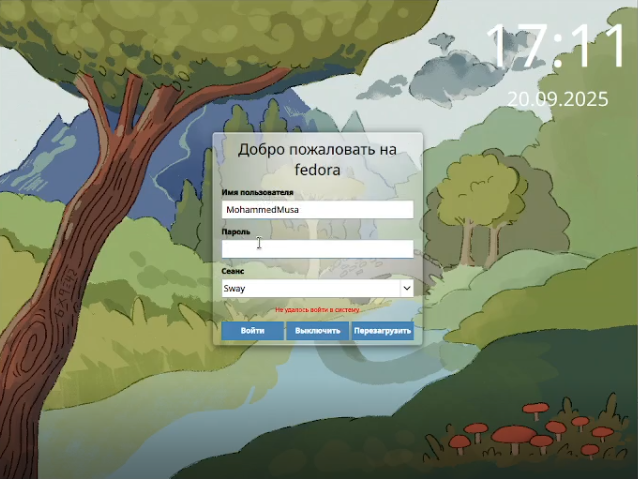
\includegraphics[width=0.9\linewidth,height=\textheight,keepaspectratio]{image/sign-in.PNG}

}

\caption{\label{fig-signin}Экран входа в систему}

\end{figure}%
\end{column}
\end{columns}
\end{block}

\begin{block}{3.2 Настройка клавиатуры}
\phantomsection\label{ux43dux430ux441ux442ux440ux43eux439ux43aux430-ux43aux43bux430ux432ux438ux430ux442ux443ux440ux44b}
\begin{columns}[c]
\begin{column}{0.7\linewidth}
\textbf{Настройка раскладок:}
\end{column}

\begin{column}{0.3\linewidth}
\begin{figure}

\centering{

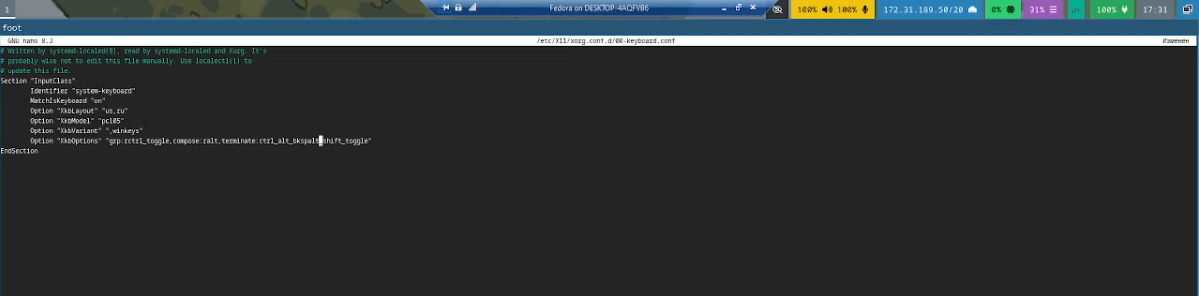
\includegraphics[width=0.9\linewidth,height=\textheight,keepaspectratio]{image/keyboard.PNG}

}

\caption{\label{fig-keyboard}Настройка клавиатуры}

\end{figure}%
\end{column}

\begin{block}{3.3 Конфигурация SELinux}
\phantomsection\label{ux43aux43eux43dux444ux438ux433ux443ux440ux430ux446ux438ux44f-selinux}
\begin{columns}[c]
\begin{column}{0.7\linewidth}
\textbf{Отключение SELinux:} - Изменение конфигурации SELinux в файле
/etc/selinux/config - Перезагрузка системы для применения изменений -
Проверка статуса SELinux командой sestatus
\end{column}

\begin{column}{0.3\linewidth}
\begin{figure}

\centering{

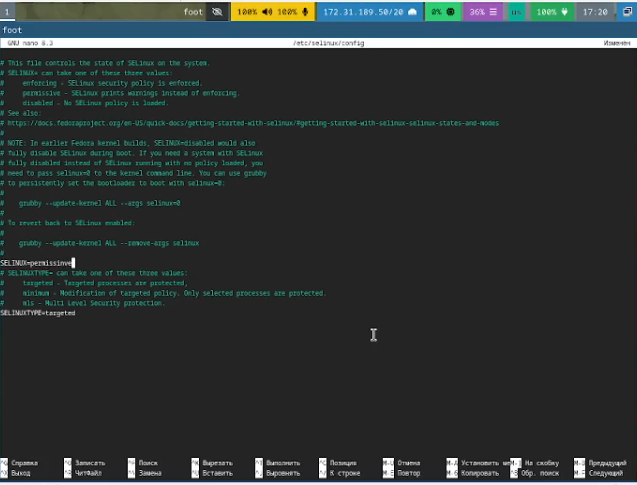
\includegraphics[width=0.9\linewidth,height=\textheight,keepaspectratio]{image/selinux.PNG}

}

\caption{\label{fig-selinux}Конфигурация SELinux}

\end{figure}%
\end{column}
\end{columns}
\end{block}

\begin{frame}[fragile]{4. Практическая работа}
\phantomsection\label{ux43fux440ux430ux43aux442ux438ux447ux435ux441ux43aux430ux44f-ux440ux430ux431ux43eux442ux430}
\begin{block}{4.1 Работа с командой grep}
\phantomsection\label{ux440ux430ux431ux43eux442ux430-ux441-ux43aux43eux43cux430ux43dux434ux43eux439-grep}
\begin{columns}[c]
\begin{column}{0.7\linewidth}
\textbf{Изучены команды поиска в логах:}

\begin{Shaded}
\begin{Highlighting}[]
\FunctionTok{dmesg} \KeywordTok{|} \FunctionTok{grep} \StringTok{"Linux version"}
\FunctionTok{dmesg} \KeywordTok{|} \FunctionTok{grep} \AttributeTok{{-}i} \StringTok{"MHz processor"}
\FunctionTok{dmesg} \KeywordTok{|} \FunctionTok{grep} \AttributeTok{{-}i} \StringTok{"CPU0"}
\FunctionTok{dmesg} \KeywordTok{|} \FunctionTok{grep} \AttributeTok{{-}i} \StringTok{"memory"} \KeywordTok{|} \FunctionTok{head} \AttributeTok{{-}n}\NormalTok{ 1}
\FunctionTok{dmesg} \KeywordTok{|} \FunctionTok{grep} \AttributeTok{{-}i} \StringTok{"hypervisor detected"}
\FunctionTok{dmesg} \KeywordTok{|} \FunctionTok{grep} \AttributeTok{{-}i} \StringTok{"MHz processor"}
\FunctionTok{dmesg} \KeywordTok{|} \FunctionTok{grep} \AttributeTok{{-}i} \StringTok{"root files"}
\end{Highlighting}
\end{Shaded}
\end{column}

\begin{column}{0.3\linewidth}
\begin{figure}

\centering{

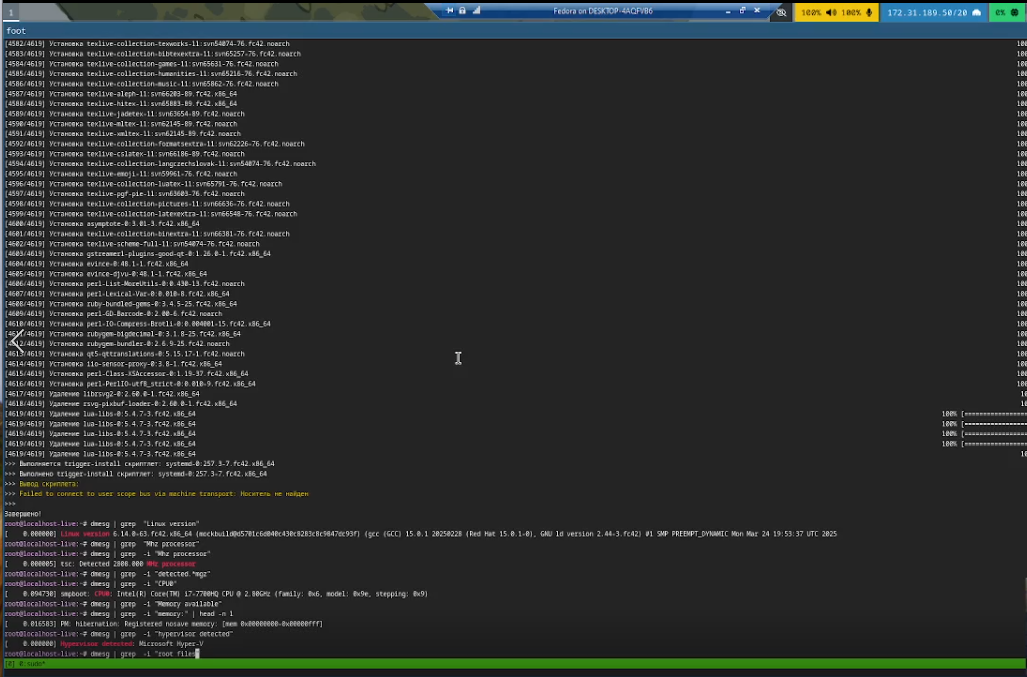
\includegraphics[width=0.8\linewidth,height=\textheight,keepaspectratio]{image/grep.PNG}

}

\caption{\label{fig-grep}Использование команды grep для поиска в логах}

\end{figure}%
\end{column}
\end{columns}
\end{block}

\begin{block}{4.2 Обновление системы}
\phantomsection\label{ux43eux431ux43dux43eux432ux43bux435ux43dux438ux435-ux441ux438ux441ux442ux435ux43cux44b}
\begin{columns}[c]
\begin{column}{0.7\linewidth}
\textbf{Загрузка необходимых инструментов:}
\end{column}

\begin{column}{0.3\linewidth}
\begin{figure}

\centering{

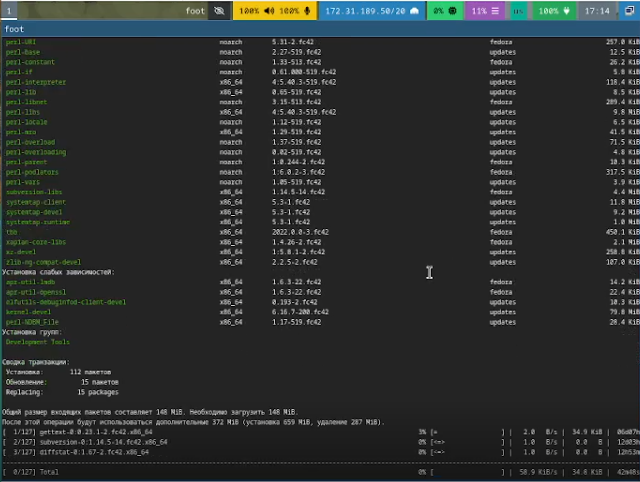
\includegraphics[width=0.9\linewidth,height=\textheight,keepaspectratio]{image/tools.PNG}

}

\caption{\label{fig-update}Загрузка необходимых инструментов}

\end{figure}%
\end{column}
\end{columns}
\end{block}

\begin{block}{4.3 Полученные навыки}
\phantomsection\label{ux43fux43eux43bux443ux447ux435ux43dux43dux44bux435-ux43dux430ux432ux44bux43aux438}
\begin{itemize}[<+->]
\tightlist
\item
  🔧 Установка и настройка Linux в виртуальной среде
\item
  👤 Администрирование пользователей и групп
\item
  ⌨️ Настройка региональных параметров (язык, клавиатура)
\item
  🔒 Управление системной безопасностью (SELinux)
\item
  🔍 Работа с текстовыми данными и системными логами
\item
  📦 Управление программными пакетами
\end{itemize}
\end{block}
\end{frame}

\begin{frame}{5. Выводы}
\phantomsection\label{ux432ux44bux432ux43eux434ux44b}
В ходе лабораторной работы были успешно выполнены все поставленные
задачи по настройке современного окружения разработки на базе Linux.
Получены фундаментальные навыки системного администрирования,
необходимые для дальнейшего изучения операционных систем и
программирования.

\textbf{Студент:} Мохамед Муса\\
\textbf{Группа:} НКАбд-05\\
\textbf{Номер:} 1032248286
\end{frame}
\end{columns}
\end{block}
\end{frame}




\end{document}
